\chapter{Nanopore Signal Analysis}
\label{cha:signal}

The primary output of third generation nanopore sequencing devices is the raw ionic current measured as a proxy signal for a DNA or RNA strand passing through the pore. 
An initial processing step of particular importance is the basecalling, translating the raw signal into the respective genomic sequence.
Common workflows such as genome assembly, structural variant or isoform detection typically rely on sequence inputs only.
However, the error rate and run time of state of the art basecalling algorithms motivate ongoing research on the processing of the raw signal itself. Furthermore, the sequencing without amplification preserves signatures of modified bases in the signal of DNA and RNA samples.
Prominent applications based on raw nanopore signals include methylation detection, barcode demultiplexing and real-time alignment for selective sequencing.
Challenges in the raw signal analysis arise from noise induced by measuring currents in pico ampere ranges and time-warping, the uncertainty of how long the molecule resides stationary in the pore before being advanced by the motor protein.


\begin{figure}[h]
    \centering
    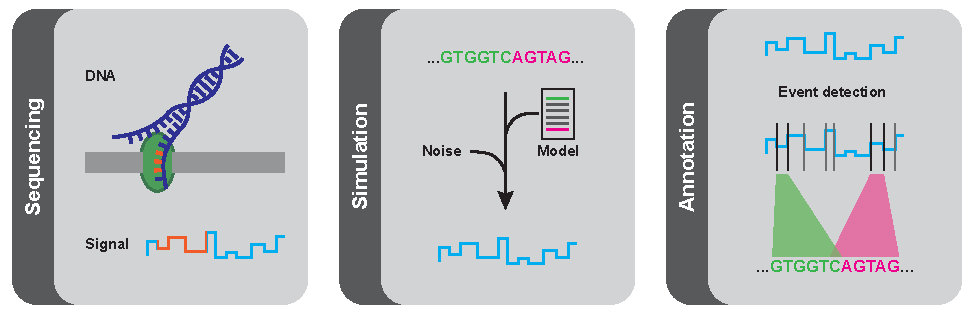
\includegraphics[width=1.0\textwidth]{figures/signal/GA.pdf}
    \label{fig:signal:ga}
\end{figure}


The following chapter serves as a transition from basic data handling and processing using \textit{Nanopype} in chapter \ref{cha:nanopype} and introduces the underlying algorithms for the signal driven repeat detection \textit{STRique} in chapter \ref{cha:strique}.
After a brief \textbf{background} in section \ref{sec:signal:background}, this chapter covers the raw signal \textbf{simulation} from known sequences in section \ref{sec:signal:simulation}. Noise and time warping are addressed by the \textbf{normalization} followed by \textbf{event detection} and \textbf{annotation} of raw nanopore reads with reference sequences in sections \ref{sec:signal:normalization} and \ref{sec:signal:alignment}.

\section{Background}
\label{sec:signal:background}

In contrast to second generation sequencing, the main output of nanopore sequencing is the ionic current measured on the device while a molecule is passing through any of its pores. The characteristics of this signal are determined by pore and chemistry version, currently R9.4.1, as released by ONT in October 2016. In March 2020 ONT released the R10.3 with a dual reader head, promising better consensus accuracy, in particular for homopolymer stretches. In terms of throughput per flow-cell, the R10 is slightly lacking behind R9 \cite{ONT2020}. Independent of the pore version, the storage of the raw signal is valuable, as constant development by ONT and researchers in the community provides enhanced readouts from existing sequencing data.

From a technical perspective, the ionic current is sampled at 4kHz and saved as a 16-Bit unsigned integer array to FAST5 files. In combination with the sequencing speed of \texttildelow450nt/s, determined by the chemistry, this results in a square wave like signal with a median of 9 measurements per nucleotide. Being a specification of the HDF5 file format, FAST5 files can be inspected with GUI and command line tools like \textit{HDFView} and \textit{h5dump}. File access from custom software is available for C/C++ programs by linking against the HDF5 library\footnote{https://bitbucket.hdfgroup.org/projects/HDFFV/repos/hdf5/browse} and from python using the \textit{h5py} package. Additionally, in order to work with most recent data sets, the VBZ compression plugin\footnote{https://github.com/nanoporetech/vbz\_compression} is required.

While the raw nanopore signal is utilized in a number of bioinformatic applications \cite{Simpson2017, Wick2018, Loose2016}, the set of methods providing frameworks is currently limited to \textit{Tombo}\footnote{https://github.com/nanoporetech/tombo}, the successor of \textit{Nanoraw} \cite{Stoiber2017} and the recently published \textit{SquiggleKit} \cite{Ferguson2019}. The motivation to develop and use custom code for the raw signal analysis is driven by the lack of sufficiently effective and customizable algorithms. For example is \textit{Tombo} hard-coded to use \textit{minimap2} alignments and writing its output in form of event tables into the FAST5 files. While technically supported by the FAST5 format, writing of analysis results into the sequencing data is generally undesirable in a multi-user environment and causes in the case of FAST5 files excessive disk usage since new, but also overwritten data sets are appended to the end of the file. \textit{SquiggleKit} so far only provides basic data indexing and signal alignment, mostly to identify barcodes in raw reads.

Publicly available, highly customizable methods in form of a generic API are still lacking, demanding the development of an in-house framework to handle raw nanopore reads. Future work aims to include advanced normalization methods like iterative re-normalization after signal alignment as described in \cite{Boza2017} and hardware acceleration comparable to the GPU implementation of a banded signal alignment in the \textit{f5c} package \cite{Gamaarachchi2020}.




\section{Simulation}
\label{sec:signal:simulation}

Third generation sequencing data can be simulated on different levels, by generating sequences with realistic read length and error rate distributions or by generating raw signal traces, ideally indistinguishable from measured ones. Simulated reads of both types are helpful to develop or test applications under controlled conditions. Two state of the art simulators are \textit{simulatION} \cite{Rohrandt2018} and \textit{deepSimulator} \cite{Li2020}, following different concepts to generate FAST5 files of simulated reads, which can be processed with common workflows. While the former utilizes exiting models of level and noise, the latter uses a LSTM neural network to generate the signal from reference sequences. Nonetheless, generation of realistic signal traces in memory can already be achieved with a pore model and an event length distribution.

A pore model describes the mapping from sequence to expected signal. The ionic current level in the nanopore is determined by the local sequence context, termed kmer. Current models utilized by e.g. \textit{Nanopolish} are build of mean and standard deviation of signal levels per 6mer. The distribution of all, in this case 4096 levels is shown in Fig. \ref{fig:signal:pm} a, emphasizing the multi-modal characteristic of the R9.4 pore.

\begin{figure}[h]
	\centering
	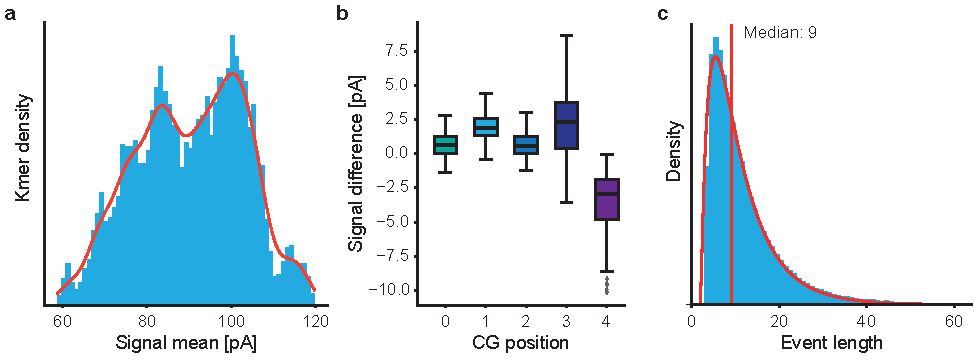
\includegraphics[width=1.0\textwidth]{figures/signal/pm.pdf}
	\captionsetup{format=plain}
	\caption[Pore model and event length]{Pore model and event lengths: \textbf{a}, Density plot and kernel density estimation of expected signal levels per kmer (k=6, n=4096, mean ionic current in pA). \textbf{b}, Expected signal difference of native and 5mC modified DNA for 6mers with single CG (n=256 per position) depending on the CG location. \textbf{c}, Event length (samples per kmer) density plot from signal alignment (red: approximation by generalized gamma distribution with a=4.3, c=0.6, shit=2, scale=0.7).}
	\label{fig:signal:pm}
\end{figure}

In general, the nanopore is sensitive for several base modifications, which are preserved when sequencing without prior amplification. A secondary pore model can be derived from sequencing e.g. 5-methylcytosine modified DNA, enabling the discrimination of native and 5mC on signal level. The model difference between native and 5mC for single-CG containing 6mers is illustrated in Fig. \ref{fig:signal:pm} b (Native and methylated model taken from \textit{Nanopolish}).

In addition to the signal level, the event length or dwell time of the molecule in the pore needs to be modeled. It is not fully understood, to which extend the behavior of the motor protein controlling the sequencing speed is a random or sequence context dependent process. Aimed solely towards the development of signal alignment methods, event lengths are randomly sampled from a generalized gamma distribution in this work. 
The distribution is derived from in-house sequencing data using the event detection described in section \ref{sec:signal:alignment} and shown in Fig. \ref{fig:signal:pm} c. The measured event median of 9 samples per 6mer matches the expected value for a sequencing speed of 450nt/s sampled at 4kHz.

With both, pore model and event length distribution, simulated raw nanopore signals can be generated from any given target sequence. The mean event level, a simulated and the corresponding stretch from a real nanopore read are depicted in Fig. \ref{fig:signal:simulation}.

\begin{figure}[h]
	\centering
	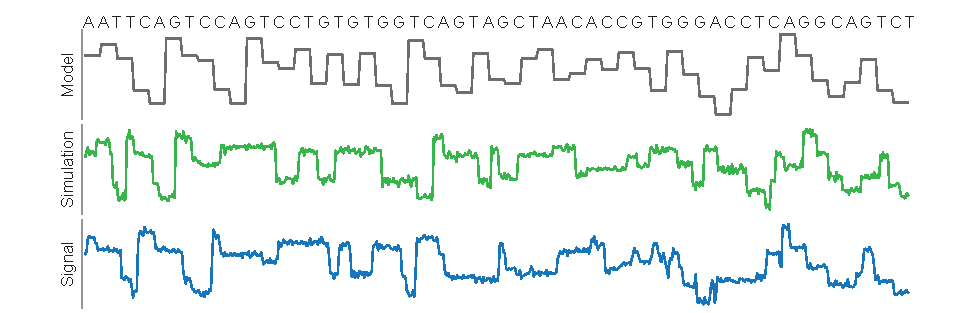
\includegraphics[width=1.0\textwidth]{figures/signal/simulation.pdf}
	\captionsetup{format=plain}
	\caption[Basic signal simulation]{Basic nanopore signal simulation from pore model and event lengths: Mean ionic current levels per kmer for short sequence (top), simulated nanopore signal with noise and random time warping (center) and raw signal fragment extracted from real nanopore read covering the same sequence (bottom).}
	\label{fig:signal:simulation}
\end{figure}

Both, the published and the proposed simplified simulation do not mirror every detail of actual sequencing data and can therefore only serve as a first approximation. Examples of missing technical artifacts are rare spikes of single values and temporarily stalled reads with hundreds of samples from the same kmer. Lastly, motor protein and analog digital converter are not synchronized, frequently resulting in measurements on the rising or falling edges between events.




\section{Normalization}
\label{sec:signal:normalization}

A robust normalization is a substantial first step during nanopore signal processing, impacting any downstream method and readout. Baseline for the following normalization is the raw ionic current measurement, saved by the sequencing software \textit{MinKNOW} as unprocessed unsigned integer with a typical numeric range from 300 to 700 (cf. Fig. \ref{fig:signal:normalization} top track). Prior to any processing we apply a median filter with a sliding window of length three to remove signal spikes and reduce the overall noise. Factors further affecting the signal levels are:

\begin{itemize}
	\item Individual offset and scale induced by the electronic circuit per pore
	\item Uneven sequence composition depending on the genomic context resulting in biased sampling from the multi modal pore model
\end{itemize}

Offset and scale for normal distributed signals can be compensated by using a z-score normalization:

\begin{equation}
	X_{norm,z-score} = \frac{X_{i} - \mu}{\sigma}
\end{equation}

Suggested by \textit{Nanoraw} \cite{Stoiber2017} and claimed to be more robust against the underlying distribution is a normalization with median offset and median absolute deviation (MAD) scale:

\begin{equation}
	X_{norm,MAD} = \frac{X_{i} - median(X)}{median(\left|X_{i}-median(X)\right|)}
\end{equation}

With regard to the signal driven repeat quantification in chapter \ref{cha:strique}, we propose a novel strategy combining a min-max and quantile normalization. Subtraction of the signals 0.025 quantile and scaling by its interquantile range is expected to be more stable, especially for biased signal distributions:

\begin{equation}
	X_{norm} = \frac{2 \cdot (X_{i} - Q_{0.025})}{Q_{0.975} - Q_{0.025}} - 1
\end{equation}

The suitability of normalization algorithms applied to real nanopore data can, in the absence of true scale and offset values, only be implicitly rated by the performance of subsequent methods. We therefore evaluate the proposed min-max normalization against the other methods on simulated signals and assess their ability to minimize the distance between simulated and normalized signal. Taking the different statistical characteristics of each normalization output into account, we first generated specific pore-models for each method, mapping the signal levels from pico ampere to e.g. the [-1:1] interval of the min-max method. We next sampled random fragments from human genome hg38 with lengths from 1kb to 10kb. Nanopore signals were simulated with event levels from each pore model and event lengths only sampled once per read to be comparable across all three methods. 

The sequence complexity is expected to influence the normalization due to a biased sampling from the multi-modal pore model. The complexity measured as observed kmers per read, divided by the total kmer count is illustrated in Fig. \ref{fig:signal:norm_methods} a. While generally rising with increased read length, none of the simulated reads contains all possible 4096 6mers.

\begin{figure}[h]
	\centering
	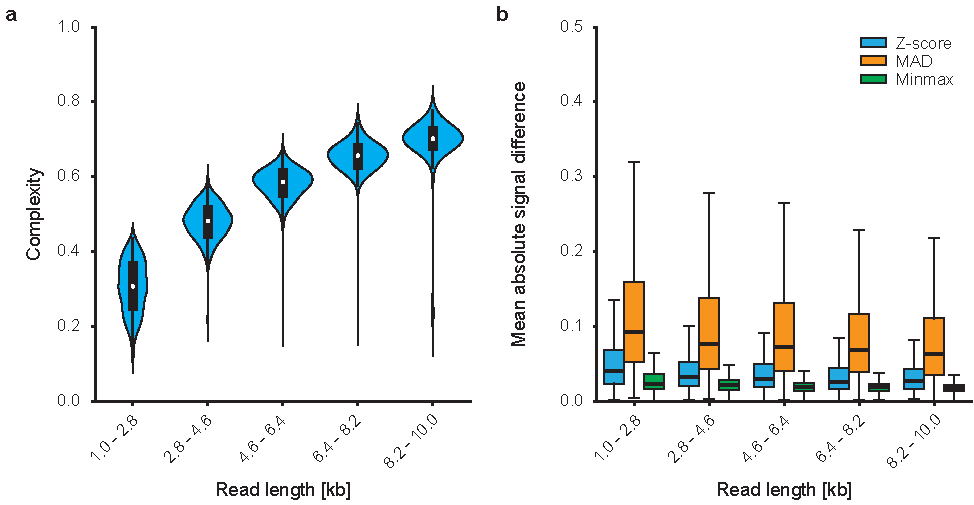
\includegraphics[width=1.0\textwidth]{figures/signal/norm_methods.pdf}
	\captionsetup{format=plain}
	\caption[Signal normalization on simulated reads]{Comparison of different normalization strategies on simulated raw nanopore signals. \textbf{a}, Sequence complexity as fraction of unique kmers per read divided by total kmer count (k=6, n = 199, 203, 213, 181, 204 reads). \textbf{b}, Mean absolute difference between simulated and normalized signal grouped by read length and normalization method. Read lengths and counts as in a, with matching event lengths used across all normalization methods. Data in a are presented as violin plots with overlayed boxplots. Data in a-b as boxplots (centerline, median; box limits, first and third quartiles; whiskers, 1.5x interquartile range).}
	\label{fig:signal:norm_methods}
\end{figure}

Ideally, a normalization method applied to a signal from a normalized pore-model is expected to be transparent. Nonetheless, the observed mean absolute differences of simulated and normalized signals show notable deviation, especially and surprisingly in the case of the MAD method (Fig. \ref{fig:signal:norm_methods} b). With overall lowest differences and especially robust against low complexity regions, indicated by less pronounced outliers, the proposed min-max normalization appears to outperform previous methods. We conclude, that the min-max normalized signal with most values in the range [-1:1] maintains the characteristics of the nanopore, is comparable to simulated reads using a pore model and is in this form used for the repeat quantification in chapter \ref{cha:strique}.

For the purpose of signal alignment and event segmentation we propose two additional steps of  histogram equalization and morphological smoothing \cite{Gonzalez2006}. Commonly used to enhance the contrast of digital images, a histogram equalization can be used to project the multi-modal distribution of mean event levels to a more uniform distribution (Fig. \ref{fig:signal:pm} a, Fig. \ref{fig:signal:normalization} bottom track). 
To further reconstruct the expected square wave like signal, we apply a morphological noise removal, specifically an opening followed by a closing with a structuring element of length three.

\begin{figure}[h]
	\centering
	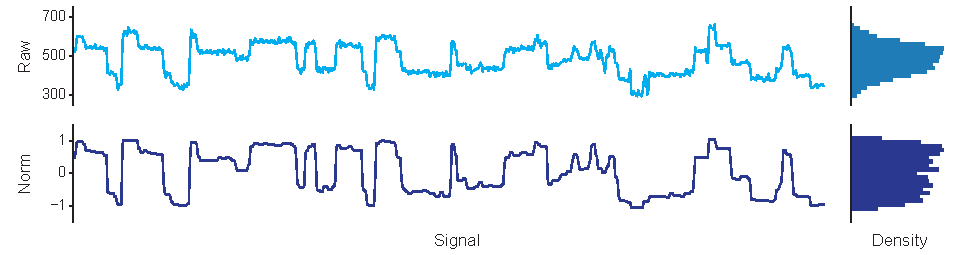
\includegraphics[width=1.0\textwidth]{figures/signal/normalization.pdf}
	\captionsetup{format=plain}
	\caption[Signal normalization and histogram equalization]{Signal normalization and histogram equalization followed by morphological noise reduction on raw nanopore signal traces. The figure shows signal segments over a 50nt window in combination with density plots of raw and normalized values over the entire read.}
	\label{fig:signal:normalization}
\end{figure}

The final result of normalized and filtered signal with a near uniform distribution of values across the full signal range is the baseline for the alignment and event detection described in the following section.




\section{Signal Alignment}
\label{sec:signal:alignment}

For applications, where neither signal nor sequence alone enable the intended readout, the sample wise annotation of raw signals with the respective reference sequence is required. Affected by the basecalling error of around 5-10\% (cf. Fig. \ref{fig:state_of_art:throughput} b), the usage of the reference sequence after read alignment is preferable over the read sequence for this purpose. The following two sections describe the \textbf{segmentation} and alignment of nanopore signals to extract any region of interest from a read and the precise \textbf{annotation} of signals with reference sequences and base modifications using Hidden Markov Models (HMM). The former is the enabling step for the latter, as HMMs become computationally very expensive with increasing numbers of hidden states and sequence lengths.




\subsection{Segmentation and Event Detection}
\label{subsec:signal:segmentation}

A semi-global signal alignment is executed between the normalized raw signal and a simulated signal with constant event length of either the complete reference span or a query region of interest within the read. Primarily to extract larger regions of interest from a raw signal, we specify a template function of the \textit{SeqAn2} \cite{Reinert2017} library to perform a distance based semi-global signal alignment. Specifically, we utilize the \textit{globalAlignment} function with a float32 data type, an affine gap penalty and the following score function:

\begin{equation}
s_{i,j} = max \left\lbrace c - \left| x_{i} - y_{j} \right| \atop 0 \right.
\end{equation}

The absolute signal difference per position is transformed into a score by subtracting it from a constant \textit{c}. The score is capped at zero as lower boundary, resulting in a fixed minimum mismatch score independent of the actual signal difference.
Gap costs within signal and simulation are configured differently. 
Both, gap open and gap extension penalty in the signal are set to a small negative value with begin and end gaps being free (semi global alignment). Gap open and extension in the simulated reference signal are scored with a penalty an order of magnitude larger. 
The rationale behind is, that gaps in the signal are expected and introduced by simulated events of length one, being stretched to the observed lengths. Gaps in the simulated reference signal are expected to by very rare and stand for sequence stretches not being observed in the raw signal.

The described approach is limited by the modeling of event lengths with affine gap costs and more severe by the quadratic time and memory complexity of the semi-global alignment with respect to the read length. Read lengths of multiple hundred kilobases make straightforward alignments in signal space increasingly ill-suited to annotate the full read. Implementations in \textit{Tombo} and \textit{Nanopolish} \cite{Simpson2017, Gamaarachchi2020} address this issue with banded alignments, without appreciating the underlying problem of an over sampled square wave like signal.

Inspired by a general concept for the discretization of time series into symbolic strings \cite{Lin2003}, we therefore further improve our signal alignment by an event compression and discretization step. Exploiting the distinct steps between events after histogram equalization and morphological noise reduction, we apply an image processing edge detection on the normalized signal using a one dimensional convolution with the kernel [-3\ -1\ 1\ 3]. Intermediate segments are summarized into an event table with their lengths and mean signal levels (Tab. \ref{tab:signal:events}). The previously described uniform distribution of signal values enables a discretization into equally represented symbols, by diving the signal range into evenly sized bins. A lookup table mapping reference kmers from the pore model to the same symbol space can be pre-computed. Lastly, any generic sequence alignment library can be used to align both symbolic sequences without handling the nanopore specific time-warping.


\begin{table}[ht]
	\centering
	\caption[Event detection and annotation]{Event table of raw nanopore signal with reference sequence annotation.}
	\label{tab:signal:events}
	\begin{tabular}{l|r|r|r|l}
		& mean & event length & seq. offset & kmer \\
		\hline 
		& \multicolumn{3}{c|}{...} &  \\
		\hline
		$ E_{n} $ &  1.332  & 15 & 3205 & AGTCCA \\
		\rowcolor{LightOrange}
		$ E_{n+1} $ &  0.981  & 22 & 3206 & GTCCAG \\
		$ E_{n+2} $ & -1.058  &  6 & 3208 & CCAGTC \\
		$ E_{n+3} $ & -1.662  & 17 & 3209 & CAGTCC \\
		$ E_{n+4} $ &  1.360  &  7 & 3210 & AGTCCT \\
		$ E_{n+5} $ &  0.664  & 33 & 3211 & GTCCTG \\
		$ E_{n+6} $ &  0.107  & 11 & 3212 & TCCTGT \\
		\rowcolor{LightGreen}
		$ E_{n+7} $ &  0.844  &  4 & 3213 & CCTGTG \\
		\rowcolor{LightGreen}
		$ E_{n+8} $ &  1.362  & 38 & 3213 & CCTGTG \\
		\hline
		& \multicolumn{3}{c|}{...} &  \\
	\end{tabular} 
\end{table}


The event alignment is implemented using the python module of the \textit{Edlib} \cite{Sosic2017} package. Based on Myer's bit-vector algorithm and with alignment path traceback in linear memory (Hirschberg's algorithm), the library supports symbol sequence alignments over alphabets of up to 256 characters. The overall sensitivity of the method depends on the edge detection threshold, resulting in an over- or under-detection of events and the size of the discretization alphabet. In this work we align event sequences represented by an alphabet of 12 characters. Furthermore \textit{Edlib} allows to extend the character equality matrix, which we utilize to treat symbols to be additionally equal with adjacent symbols in terms of the signal level they represent.

A small extract of the resulting event annotation is shown in Table \ref{tab:signal:events}. Highlighted are a row followed by a missed event (deletion, orange) and two rows belonging to the same reference kmer (insertion, green). Taken together, the event detection and alignment maps 90\% of the events to a unique kmer, 5\% are over segmented and the remaining 5\% are distributed to the most critical errors of single and consecutive reference kmers without signal observations.

The above signal alignment enables reference guided extraction of any region of interest from long nanopore reads. Yet, for the analysis of base modifications encoded into the signal or regions diverging from the reference genome, a more sophisticated model is needed.




\subsection{Annotation}
\label{subsec:signal:annotation}

Already proposed for the analysis of nanopore signals from previous pore generations, Hidden Markov Models are a powerful resource to map signal onto sequence features \cite{Schreiber2015}. In contrast to the discrete emission distributions for e.g. sequence motive detection, the hidden states model in this case the sequence context depending signal observed in the pore, overlayed by Gaussian distributed noise.

The first generation of basecalling algorithms provided by ONT used HMMs with hidden states derived from kmer signal levels and all possible transitions between consecutive overlapping kmers. The Viterbi path through such a model is the most likely state- and thus genomic-sequence given the observed signal. Whereas outperformed by recurrent neural networks for basecalling, HMMs still provide state of the art performance for base modification detection such as in \textit{Nanopolish}. For the repeat analysis in chapter \ref{cha:strique} we use profile Hidden Markov Models closely following the concept of modular blocks described in \cite{Schreiber2015}.

Starting of with a target sequence, a series of match states from overlapping kmers and with normal distributed signal emissions forms the expected path through the model. Additional insertion states with uniform emission distributions over the whole signal range compensate observations outside of the match state distributions. Lastly, silent deletion states allow the model to skip parts of the profile sequence without corresponding observations in the signal (Fig. \ref{fig:strique:count_hmm} a, b).

\begin{figure}[h]
	\centering
	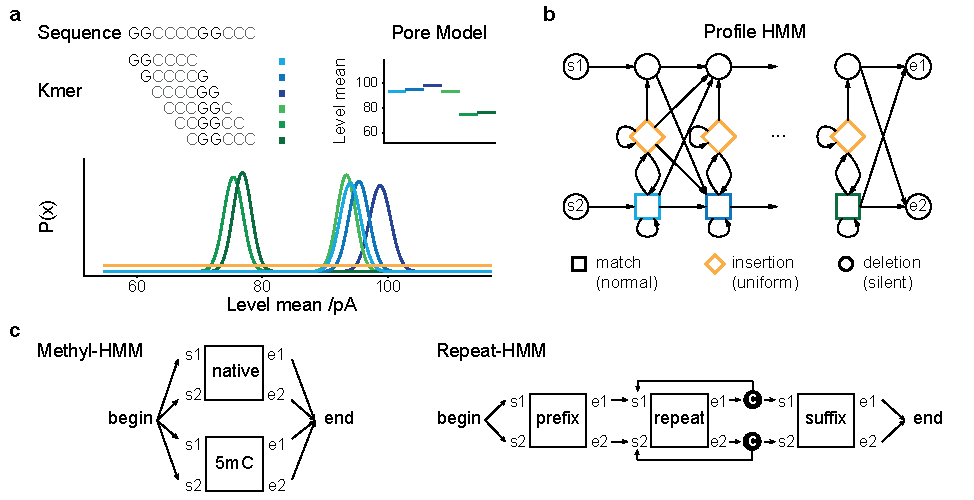
\includegraphics[width=1.0\textwidth]{figures/signal/count_hmm.pdf}
	\captionsetup{format=plain}
	\caption[Nanopore signal alignment with HMMs]{Nanopore signal alignment with HMMs: \textbf{a}, Consecutive overlapping kmers from profile sequence with corresponding pore model levels and expected emission distributions in the pore. \textbf{b}, Nanopore signal profile HMM with normal distributed match states and uniform distributed insertion states. \textbf{c}, A methylation detection HMM with emission distributions for native and 5mC modified DNA. A compound profile HMM of prefix, a single repeat and the suffix sequence with dummy states counting transitions through the repeat module.}
	\label{fig:strique:count_hmm}
\end{figure}

Simply chained by single transitions to the four outer silent states, the modular profile HMM blocks can be used to build more complex architectures as illustrated in Fig. \ref{fig:strique:count_hmm} c. 

The first example shows a possible base modification detection architecture with two profile HMM components derived from the same sequence, but with emission distributions centered around expected signal levels of native and for instance 5-methylcytosine modified DNA. Computing the log-probability and Viterbi path through this model yields the most likely hidden state sequence of one branch given an observed nanopore signal.
The second example addresses the case of heterogeneous genomic regions, where reference and sequenced individual diverge. In-depth introduced in the following chapter, short tandem repeats are 2-8nt sequence fragments with varying repetition counts per individual. The illustrated compound profile-HMM is anchored by stable and known genomic prefix and suffix sequences, framing a single instance of the repeat. Feedback transitions around the repeat enable the model to adjust to any repeat length. In this case, the Viterbi path as most likely state sequence given the observed signal is used to quantify the length of the tandem repeat.




\section{Summary}
\label{sec:signal:summary}

Taken together, this chapter introduces signal processing methods required to integrate the genomic sequence with additional information encoded in the raw nanopore signal. Normalization methods reversing scale and offset induced by the sequencer have been compared and form the backbone for subsequent analysis steps. The advancement of existing banded signal alignment algorithms by event compressed symbolic sequences makes this framework fast and memory efficient. Lastly profile Hidden Markov Models are introduced as universal but also computationally most expensive method. In the following chapter, above methods are applied to analyze the biological phenomena of expanded short tandem repeats in clinical relevant disease contexts.






